% overview.tex
% RICHARD NOTE:
%   Original version:
%      Planning/ShortProjectEvaluations/2013-08-MeBradyEtAl-MarginalizedPE/overview.tex
\documentclass[twocolumn,prd,nofootinbib]{revtex4}
%\newcommand\ForRichardOnly[1]{#1}
\newcommand\ForRichardOnly[1]{}
\usepackage{verbatim}
\usepackage{color}     % color text
\usepackage{framed}
\definecolor{shadecolor}{gray}{0.95}
\usepackage{amsmath}
\usepackage{graphicx}  % extend graphics
\usepackage{tabularx}
\usepackage{wrapfig}   % wrap text around figures, if desired
\usepackage{hyperref}

% Standard LAL, LALAPPs links
\newcommand\LALDocsMain{\href{http://www.lsc-group.phys.uwm.edu/lal/slug/nightly/doc/lsd-nightly.pdf}{LALDocs}}
%\newcommand\LALappsDocsMain{\href{http://www.lsc-group.phys.uwm.edu/~saikat/doc/lalapps.pdf}{LALapps docs}}
\newcommand\LALappsDocsMain{\href{http://www.lsc-group.phys.uwm.edu/lal/slug/nightly/doc/lalapps-nightly.pdf}{LALapps docs}}
\newcommand\LALDocsSource[1]{\href{http://www.lsc-group.phys.uwm.edu/cgit/lalsuite/tree/#1}{#1}}
\newcommand\LALDocsSourceInline[2]{\href{http://www.lsc-group.phys.uwm.edu/cgit/lalsuite/tree/#1}{{\tt #2}}}

% BONUS TOOLS

\newcommand\editremark[1]{{\color{red} #1}}

\newcommand\unit[1]{\, {\rm #1}}
\newcommand\aap{A\&A}
\newcommand\apss{APSS}
\newcommand\aaps{AAPS}
\newcommand\apjs{ApJ S}
\newcommand\aj{AJ}
\newcommand\apjl{ApJL}
\newcommand\mnras{MNRAS}
\newcommand\pasp{PASP}
\newcommand\araa{ARA\&A}
\newcommand\physrep{Phys. Rep.}
\newcommand\aapr{AAPR}
\newcommand\nar{NAR}  % New astronomy reviews

\newcommand\Y[1]{Y^{(#1)}{}}
% GR tools
\newcommand\prederiv[2]{{}^{(#1)}#2}
\newcommand\dualBack{*}
\newcommand\dualForward{\star}
\newcommand\avL{\left< {\cal L}_{(a} {\cal L}_{b)} \right>}
\newcommand\WeylScalar{{\psi_4}}
\newcommand\WeylScalarFourier{{\tilde{\psi}_4}}
\newcommand\mc{{{\cal M}_c}}
% QM TOOLS
\newcommand\qmstate[1]{\left|#1\right \rangle}
\newcommand\qmstateKet[1]{\left\langle#1\right|}
\newcommand\qmstateproduct[2]{\left\langle#1|#2\right\rangle}
\newcommand\qmoperatorelement[3]{\left\langle#1\left|#2\right|#3\right\rangle}
\newcommand\qmoperator[1]{{\bf #1}}


\begin{document}

\title{PE by Monte Carlo}
\author{R. O'Shaughnessy}
\author{E. Ochsner}
\author{C. Pankow}
\author{P. Brady}
\author{H. Qi}
\begin{abstract}
Notes. Main content in white.  Gray sidebars are ``footnotes'': implementation tricks and comments to be skipped on a
first read.
\end{abstract}
\maketitle
\tableofcontents
\part{Notes for group}
\nocite{gwastro-HarryFairhurst-CoherentTargetedSearch}
% Keppel http://adsabs.harvard.edu/cgi-bin/nph-data_query?bibcode=2012arXiv1208.2340K&link_type=ABSTRACT

\section{Stage 0: What are we calculating}

\subsection{The reduced likelihood}
\noindent \textbf{Gravitational wave signal}: Paramters $\lambda,\theta$ for $\lambda$ intrinsic parameters (slow) and
$\theta$ extrinsic parameters (fast).  The code provides $h(t|\lambda,\theta)$ in the Earth's barycenter or, more
usefeul, $h_{lm}$, a spin-weighted spherical harmonic decomposition relative to the emission direction $\hat{N}$
\begin{shaded}
\begin{itemize}
\item $h(t)=h_+-i h_\times$ is a complex strain unless explicitly indicated otherwise.   Capital letters $H$ denote
  quantities in a particular detector's data stream.  The hatted quantity $\hat{H}_k$ is the measured strain data in the
  $k$th detector.
\item All operations respect polarization symmetry and time translation.  Under a rotation by $\psi$ around the
  propagation direction, the waveform transforms as
\[
h' = h \exp(-2i \psi)
\]
\item The source propagation direction away from the source is $\hat{n}(\theta_{JN},\phi_{JN})$ where
  $\theta_{JN},\phi_{JN}$ are the angles of the propagation direction relative to the total angular momentum vector (at
  some time) $J$; the projection of $J$
  onto the plane of the sky is $\psi_J$.  The spin-weighted
  spherical harmonic decomposition is 
\begin{eqnarray}
\label{eq:def:hSpinWeightEmissionDirection}
h(t|\lambda,\theta) = \sum_{lm} h_{lm}(t|\lambda) e^{-2i\psi_J}\Y{-2}_{lm}(\theta_{JN}\phi_{JN})
\end{eqnarray}
Note $h_{lm}$ depends only on intrinsic parameters.  (Implicitly, $h_{lm}$ also depends on our choice of reference
frequency, typically 100 Hz.).  Coefficient functions $h_{lm}$ are provided in
\cite{gw-astro-mergers-approximations-SpinningPNHigherHarmonics}; the theory underlying orbital phase generation is
summarized in  \cite{gw-astro-PN-Comparison-AlessandraSathya2009}, etc.
\item The sky location is $\hat{n}=\hat{n}(\delta,\alpha)$ (i.e., RA and DEC angles).  we do not have to do sky location
  conversions ourselves.
\item Fourier sign convention is as follows, consistent with \cite{gwastro-mergers-nr-Alignment-ROS-Polarization}
\begin{eqnarray}
h(t) = \int \frac{d \omega}{2\pi} \; e^{-i\omega t} \tilde{h}(\omega) \\
\tilde{h}(2\pi f) = \int dt e^{i 2\pi f t} h(t)
\end{eqnarray}
In the common case that  $h = Ae^{-i\Phi(t)}$ with $\Phi$ increasing monotonically, the fourier transform $\tilde{h}(f)$ will be dominated by
positive-frequency components
\end{itemize}
In practice $h(t)$ is timesampled at some fixed rate for its entire duration.  The signal duration is dominated by
low-frequency content.
\end{shaded}


\noindent \textbf{Response of each detector}: Each detector has a response function which returns some $H_k(t)$, the
``strain'' function of that detector.  No matter how complicated the response, it must satisfy time-translation symmetry and spin-weight-$-2$ symmetry.
 \emph{Generic} detector response must account for arbitrary frequency
content at each time and requires slow calculations to carefully propagate signals with $f\simeq f_{FSR}$.  

In the
\emph{long wavelength limit} the response can be approximated using some $F_+,F_\times(t)$:
\begin{align}
H_k(t) &=F_{+,k}(t) h_+(t-\vec{x}_k(t)\cdot \hat{k}) + F_\times(t) h_\times(t-\vec{x}_k(t)\cdot \hat{k}) \\
 &= \text{Re}(F_++i F_\times)_k h(t-\vec{x}_k(t)\cdot \hat{k}) \\
 &=  \frac{F h }{2} + \frac{F^*h^*}{2} \equiv (Fh  + F^*{\cal I} h)/2
\end{align}
where $-\hat{k}$ points toward the sky location, \emph{opposite} to the direction of propagation $\hat{k}$; where $F=F_++i F_\times$;
where $F_{+,\times}$ are calculated as $F_+(t)=e_+^{ab}d_{ab}(t)/2$ and follow by contracting a unit tensor with the time-dependent geometry tensor of each
interferometer; where self-evident dependence on $t$ and $t-\hat{k}\cdot \vec{x}_k$ has been suppressed; and
where ${\cal I}$ is the (complex-antilinear!) complex conjugation operation in time.   
\begin{shaded}
\noindent \textbf{A ``complex conjugate''}: What is  ${\cal I}$? I want to take fourier transforms of the complex
conjugate of a  complex function of time
unambiguously.  So ${\cal I}$ is the ``complex conjugate in time'' operation:
\begin{align}
{\cal I}\tilde{h}(\omega) &\equiv \int e^{-i\omega t} h(t)^* dt  = [\tilde{h}(-\omega)]^* \\
{\cal I} p h &= p^* {\cal I} h \\
(a,{\cal I} b) & = (b,{\cal I}a) = 2 \int_{-\infty}^{\infty} df \frac{[\tilde{a}(f)]^*[\tilde{b}(-f)]^*}{S_h(|f|)}\\
 &= ({\cal I} a,b)^*
\end{align}
which trivially satisfies ${\cal I}^2=1$.  Remember ${\cal I}$ is \emph{not} linear, as ${\cal I} i h = -i {\cal I} h$
and hence ${\cal I}F=F^*{\cal I}$.  
Because of how it prefers time, however, it will \emph{not} conjugate  $i\omega$ (i.e., time translations):  if $h'(t)=h(t-\Delta t)$, then 
\begin{eqnarray}
\tilde{h}' = e^{-i\omega \Delta t}\tilde{h} \qquad {\cal I}\tilde{h}' = e^{-i\omega \Delta t} {\cal I}\tilde{h}
\end{eqnarray}


\noindent \textbf{Complex inner products}: I want to use a hilbert space, allowing complex arguments.  My preferred inner product is
therefore complex-valued; see \cite{gwastro-mergers-HeeSuk-FisherMatrixWithAmplitudeCorrections}. 
\end{shaded}

\begin{shaded}
\noindent \textbf{Evaluating the response functions}
The beampattern operations $F_{+,\times}$ are applied in the time domain. The translation to each detector position is
applied using a set of short fourier transforms.  The cost to construct $H_k$ from $h$ is therefore  $\simeq N_{samp}\ln
N_{samp}$ for $N_{samp} = \ln
T/\Delta t$.

For a sufficiently short-duration source, both the beampattern functions and detector positions can be approximated by
constants.  Strictly, this limit does not hold for binary neutron stars.  As a first approximation, however, we can
probably assume  the fourier transform $\tilde{H}_k[h]$ can be re-expressed as 
\begin{eqnarray}
\tilde{H}_k = \frac{e^{i\omega \hat{k}\cdot \vec{x}_k}}{2}\left[ 
   F_k  \tilde{h} + F_k^* {\cal I} \tilde{h} 
 \right]
\end{eqnarray}
[Physically, equation reflects a common time translation applied to two basis signals appearing in  $\text{Re} F h$.]
\end{shaded}


\noindent \textbf{Likelihood}: Each detector has a noise power spectrum $S_{h,k}$, assumed known and
stationary, defining an inner product $\qmstateproduct{a}{b}_k \equiv 2 \int_{-\infty}^\infty  a^*(f)b(f)/S_{h,k}(f)$ on
complex-valued functions $a,b$ of time.  Each detector has strain data $\hat{H}_k(t)$.  We evaluate the following likelihood ratio for each element
\begin{eqnarray}
-2\ln L_k &= \qmstateproduct{H_k-\hat{H}_k}{H_k-\hat{H}_k}_k - \qmstateproduct{\hat{H}_k}{\hat{H}_k}_k \\
  &= \qmstateproduct{H_k}{H_k}_k - 2 \text{Re} \qmstateproduct{H_k}{\hat{H}_k}_k 
\end{eqnarray}
The total likelihood is the product of individual detectors' likelihoods:
\begin{eqnarray}
\ln L &\equiv \sum_k \ln L_k  = \ln L_{\rm model} + \ln L_{\rm data} \\
\ln L_{\rm model} &\equiv -\frac{1}{2} \sum_k \qmstateproduct{H_k}{H_k}_k \equiv - \rho^2/2 \\
\ln L_{\rm data} &\equiv  \sum_k \qmstateproduct{H_k}{\hat{H}_k}_k 
\end{eqnarray}
\ForRichardOnly{
\begin{shaded}
\textbf{Efficiency of terms?}: As described below, the two terms in the log likelihood
\begin{itemize}
\item \emph{Model-only term}: This time-translation-independent $L_{\rm model}$ can be efficienly calculated from $\tilde{h}$ in the
  barycenter, for any sky location [Eq. \editremark{X}], from an O(N) operation.  To get $\tilde{h}$ in the barycenter for
  an arbitrary \emph{emission} direction, we need to sum over $\tilde{h}_{lm}(f)$ via
  Eq. (\ref{eq:def:hSpinWeightEmissionDirection})
\item \emph{Data term}: The other term can be efficiently computed for all times, sky locations, and emission directions
  by archiving $\qmstateproduct{h_{lm}\exp(-i\omega t)}{\hat{H}_k}$ timeseries [Eq. (\ref{eq:IndividualDetectorLikelihoodTimeseries:ViaSpinWeightBasis})].
\end{itemize}
\end{shaded}
}

\begin{widetext}
\begin{shaded}
\noindent \textbf{Reorganize?}
Using the notation in  \citet{gwastro-mergers-HeeSuk-CompareToPE-Aligned}, we define 
\begin{eqnarray}
-2 \ln L &\equiv \rho^2 - 2 \sum_k \qmstateproduct{H_k}{\hat{H}_k}
\end{eqnarray}
The first term is time-translation invariant and ``easy'' to evaluate ``once and for all'' -- see later tricks with
$h_{lm}$.   The second term can be resummed by substituting the value of $H_k$ in terms of translations, beampatterns,
and $h(t)$ at the barycenter.  So...


\noindent \textbf{Coherent likelihood for a stationary network}: Assume $\vec{x}_k$ and $F_k$ are  stationary, so
$\tilde{H}_k(f)$ is easily evaluated and substituted: 
%\editremark{fix definitions: be consistent with old notation; make sure I include both terms}
\begin{align}
\label{eq:def:BarycenteredInnerProductWithData}
\sum_k \qmstateproduct{H_k}{\hat{H}_k}_k 
& = 
 \sum_k \frac{1}{2}\left [ \qmstateproduct{ F_k h +  F_k^*{\cal I}h}{e^{i\omega \hat{k}\cdot \hat{x}_k} \hat{H}_k}_k
 \right]
= \text{Re} \qmstateproduct{h}{{\cal S}}_{\rm ref} \\
\tilde{{\cal S}}(f) &= \sum_k \hat{H}_k(f) \frac{S_{\rm ref}}{S_{k}} F_k^* e^{-i\omega \hat{k}\cdot \vec{x}_k} \equiv \sum_k {\cal S}_k\\
{\cal S}(t) &= \sum_k F_k^* H_k(t+\vec{x}_k\cdot \hat{k}) \quad \text{if all detectors identical}
\end{align}
The inner product $\qmstateproduct{.}{.}_{\rm ref}$ uses a reference PSD; exact equality holds for any choice, including
a geometric mean PSD or a single reference interferometer:
\begin{eqnarray}
S_{\rm ref}^{-1} = \frac{1}{N_{\rm det}} \sum_k S_{k}(f)^{-1} \quad ;\text{or} \quad  S_{\rm ref} = S_1
\end{eqnarray}
%
In this form, the translated detector data carries all information about the sky location; no information about the
source is used.  The data from each detector is \emph{barycentered} by first applying the \emph{inverse} time
translation operation; then the beampattern response and detector PSD, as a weight.
%

Similarly, the signal amplitude can be expressed using barycentered quantities.  Taking care to allow for different PSDs
in different detectors, we find
\begin{align}
\label{eq:CalculateRhoFromBarycenterStrain}
\rho^2& \equiv \sum_k \qmstateproduct{H_k}{H_k}_k 
 =  \frac{1}{2}\qmoperatorelement{h}{\sum_k F_k^* F_k\frac{S_{\rm ref}}{S_k}}{h}_{\rm ref} 
 + \frac{1}{4}\qmoperatorelement{h}{\sum_k F_k^* F_k^* \frac{S_{\rm ref}}{S_k}}{{\cal I} h}_{\rm ref}  
 + \frac{1}{4}\qmoperatorelement{{\cal     I}h}{\sum_k F_k F_k \frac{S_{\rm ref}}{S_k}}{h}_{\rm ref}  \\
&\equiv  \qmoperatorelement{h}{\sigma}{h}_{\rm ref}  + \frac{\text{Re}}{2} \qmoperatorelement{h}{\zeta^*}{{\cal I}
   h}_{\rm ref}
\end{align}
where the last expression implicitly defines the operators $\sigma(f|\hat{k}), \zeta(f|\hat{k})$:
\begin{eqnarray}
\sigma \equiv \frac{1}{2} \sum_k |F_k|^2 \frac{S_{\rm ref}(f)}{S_k(f)} 
\qquad 
\zeta \equiv \sum_k F_k F_k \frac{S_{\rm ref}(f)}{S_k(f)} 
\end{eqnarray}

\noindent \textbf{Why do we care, mark 1}: This operation [Eq. (\ref{eq:def:BarycenteredInnerProductWithData})] allows us to quickly explore any individual sky location.  And to
explore alternative sky locations (via all possible time translations of the raw data): just reconstruct ${\cal S}$ from
the raw data streams slightly differently.   And to reduce the number of FFTs we need to perform for time translation:
having constructed ${\cal S}$, it needs to be fourier transformed only once to make the network SNR timeseries.

\noindent \textbf{Why do we care, mark 2}: Suppose we tabulate $\tilde{h}_{lm}(f)$. We can efficiently generate
$\tilde{h}$ for any emission direction [Eq. (\ref{eq:def:hSpinWeightEmissionDirection})] via an order N operation
($\tilde{h}$ depends only on emission direction, not sky position),
then efficiently generate $\rho^2$ for any sky location via an O(N) operation [the inner product with these
  sky-position-dependent operations].  

To be even more efficient, we can pre-tabulate the $\qmstateproduct{h_{lm}}{h_{l'm'}}$, which depend only on $\lambda$
and the $k$th detector PSD, and reconstruct $\rho^2$ algebraically:
\begin{subequations}
\label{eq:ComputeRhoViaInnerProductMatrix}
\begin{align}
{\color{blue} U_{k,lm,l'm'}(\lambda)}& = \qmstateproduct{h_{lm}}{h_{l'm'}}_k \\
V_{k,lm,l'm'}(\lambda)& = \qmstateproduct{{\cal I}h_{lm}}{h_{l'm'}}_k \\
\ln L_{\rm model}(\lambda|\hat{n},\hat{k},\psi_J,d) &=
   -\frac{(d_{\rm ref}/d)^2}{2}\sum_k
\left[
{\color{blue}
 \frac{1}{2}|F_k(-\hat{k})|^2 U_{k,lm,lm'}(\lambda)[\Y{-2}_{lm}(\hat{n})]^*\Y{-2}_{l'm'}(\hat{n})
}
 \right. \nonumber \\ & \left.
 {\color{blue}
+
 \frac{1}{2} \text{Re} V_{k,lm,l'm'} e^{-4i\psi_J}F_k^2 \Y{-2}_{lm}(\hat{n})\Y{-2}_{l'm'}(\hat{n})
}
\right]
\end{align}
\end{subequations}

\noindent \emph{Implementation tricks}: To minmize confusion, I recommend evaluating ${\cal I}h_{lm}(t)$ in the time
domain and fourier transforming it, so it has exactly the same code path as $\tilde{h}_{lm}(f)$; for speed you can use
${\cal I}\tilde{h}_{lm}(f) = h_{lm}(-f)^*$ if you are careful.

For nonprecessing binaries $\tilde{h}_{lm}(-f)^*=(-1)^lh_{l,-m}$ and therefore $V_{k,lm,l'm'} = (-1)^l U_{k,l-m,l'm'}$
\end{shaded}

\end{widetext}




\noindent \textbf{Reduced likelihood}: The reduced likelihood combines all detectors and integrates over all prior
volume:
\begin{eqnarray}
{\color{blue} L_{\rm red} = \int p(\theta) d\theta \prod_k L_k = \int p_s(\theta) d\theta \frac{p}{p_s}\prod_k L_k }
\end{eqnarray}
where $p_s$ is our sampling prior.  Specifically, if $d_{\rm max}$ is the maximum distance allowed and $T_{window}$ the
time window, the reduced integral has the form (for \textbf{Euclidean cosmology})
\begin{eqnarray}
L_{\rm red} = \int \frac{dt}{T_{\rm window}} \frac{d^2 dd d\Omega_{sky} }{V_{\rm max}} \frac{d\Omega_{\rm
    emit}}{4\pi} \frac{d\psi}{\pi} L
\end{eqnarray}



\ForRichardOnly{
\subsection{Stage 0: Marginalize in time}
\noindent \textbf{Rationale}: For long (BNS) signals, constructing the waveform for a fixed propagation direction is expensive, because of the cost of time translation to
each site.  Let's get the most out of each sky location


\noindent \textbf{Method: FFT translation?}: The fourier transform of the inner product provides automatic time
translation on a discrete timesample grid $t_p = t_o + n\Delta t$, using a discrete FFT approximation to
\begin{align}
-2 \ln L_k(t_p)& = \qmstateproduct{H_k}{H_k}_k + 4\text{Re}\int_{-\infty}^\infty df 
  \frac{e^{-i2\pi f t_p}\tilde{H}_k(f)\tilde{\hat{H}}_k(f)}{S_{h,k}(f)} \\
-2 \ln L(t_p) & = \rho^2 -4 \text{Re}\int_{-\infty}^{\infty} df e^{-i2\pi f t_p} \sum_k\frac{\tilde{H}_k(f)\tilde{\hat{H}}_k(f)}{S_{h,k}(f)} \\
&\equiv \rho^2 - 2 \rho \hat{\rho}(t)
\end{align}
where the first term  $\qmstateproduct{H_k}{H_k}_k$ must be independent of time and where the second term defines
$\hat{\rho}(t)$, a function of time, the data, and the template.   Marginalization over event time therefore corresponds to using these sample points to evaluate
the integral:
\begin{eqnarray}
\int dt L p_t(t)  = \frac{1}{T_{window}} \int_{t_{start}}^{t_{start}+T_{window}}dt  e^{\ln L}
\end{eqnarray}

\begin{shaded}
\noindent \textbf{Quadrature}: A typical low sample rate (few kHz) is often not enough to
evaluate the integrand in the likelihood with a naive (box) quadrature.  Very high sampling rates \textbf{or interpolating the
  integrand $L_k$  and integrading accordingly}  are needed to integrate the likelihood.

We can use any intelligent quadrature method we want for the integral -- including locally interpolating the integrand
$L$ to make a locally continuous function and integrating with any quadrature desired. 

%For speed, we may want a \emph{rejection approximation}: approximate the integrand as \emph{zero} if the max log
%likelihood is less than a certain value, or the posterior is distributed widely in time.  (Not clear if this saves us
%much: we have already done the FFT.)

\noindent \textbf{${\cal S}$ and coherent data}:  If organized intelligently, only one inverse FFT is needed to
construct $\hat{\rho}(t)$ for each sky location.  [An even better scheme uses only one inverse FFT per detector for
  \emph{all} sky locations...see $h_{lm}$ later.]

%% \noindent \textbf{Massively less than unity?}: For a physical source,  the log likelihood will be massively less than
%% unity almost everywhere.   If we just want reliable parameter estimates
\end{shaded}


\subsection{Stage 1: Marginalize in time and polarization angle}

\noindent \textbf{Rationale}: As above.
%
In GW searches, time and polarization phase marginalization is done simultaneously.  At each timesample, we expected we could
 marginalize \emph{analytically} over polarization phase, with a bessel function.

That's not true.

\noindent \textbf{Challenges}: In general the detector network and source (aka data) have preferred orientations.  These
orientations need not agree.  
\begin{shaded}
\noindent \textbf{Template amplitude}: Using the $\sigma,\epsilon$ notation of \citet{CutlerFlanagan:1994}, the signal amplitude term has the form $\rho^2 = \sigma
\rho_0^2(1+\epsilon \cos 4(\psi-\psi_0))$ where $\rho_0^2$ is the amplitude of a source directly overhead a single
detector and $\sigma,\epsilon$ are derived from the beampattern functions:
\begin{eqnarray}
C_{\lambda \lambda'}&=& \sum_k \begin{bmatrix}
F_+^2 & F_+F_\times \\
F_\times F_+ & F_\times^2
\end{bmatrix}\\
&=& \sum_k [P_k : \hat{e}_\lambda(\hat{n})] [P_k : \hat{e}_{\lambda'}(\hat{n})]  \nonumber \\
& =& \sigma U\begin{bmatrix} (1+\epsilon) & 0 \\ 0 & 1-\epsilon \end{bmatrix} U^{-1} 
\end{eqnarray}
where $U$ is a unitary transformation that diagonalizes $C$.

\noindent \textbf{Response against data}: By contrast, for a fixed data set, the second term in the likelihood
necessarily transforms like $h$: purely sinusoidally in polarization angle
\begin{eqnarray}
\rho \hat{\rho} = A \cos 2\psi + B \cos 2 \psi
\end{eqnarray}
\noindent \textbf{Marginalizing?}: If this were the only term in the likelihood -- for example, for an isotropic network
--  we could marginalize exactly: \textbf{BUT THIS IS NOT TRUE}
\begin{align}
\ln L  &= [\ln L]_c \cos 2\psi + [\ln L]_s \sin 2\psi = \ln L_0 \cos 2(\psi-\psi_0)  \\
\ln L_0 &= \sqrt{[\ln L]_c^2+[\ln L]_c^2} \\
\int_0^{\pi}\frac{ d\psi}{\pi} L &= \frac{1}{\pi}I_0(\ln L_0)
\end{align}
In general $\rho$ depends on $\psi$, so we can't: both $\cos 2\phi$ and $\cos 4\psi$ appear in the exponential, unless
the network has $\epsilon=0$ (i.e., equal sensitivity to both polarizations).
\end{shaded}



\noindent \textbf{Method: Phase alone}: We know how to evaluate all the terms in the likelihood given 4 quadrature
points at $0,\pi/4, \pi/8, 3\pi/8$.  We could hardcode the integral
\begin{eqnarray}
\int_0^{\pi}\frac{ d\psi}{\pi} e^{\ln L}
\end{eqnarray}
using values at these 4 points.   Or otherwise provide a fast way to evaluate the 1d integral, given the known form of
$\rho$ and $\qmstateproduct{h}{{\cal S}}$ veruss $\psi$

\noindent \textbf{Method: Phase and time integral}: Marginalizing over phase can be performed at each $t_p$ using the
archived values  $L(t_p, \psi)$ computed by fourier transforming the signal for several $\psi$...or by other methods.
\begin{eqnarray}
\int \frac{dt}{T_{\rm win}} \int \frac{\psi}{\pi}L
\end{eqnarray}




\subsection{Stage 2: Marginalize in time, polarization angle, and distance }

\noindent \textbf{Rationale}: As above.

\noindent \textbf{Challenges}: No analytic simplifications possible here or henceforth 

\noindent \textbf{Principle}: In each $\ln L_k$  are terms that scale quadratically with $1/d$
($\qmstateproduct{H}{H}$) and terms that scale linearly with $1/d$ ($\qmstateproduct{H}{\hat{H}}$).  If we pick one
reference value, we can rescale all terms in $L$ analytically:
\begin{align}
-2 \ln L &= \rho_{\rm ref}^2 (d_{ref}/r)^2  - 2 (d_{\rm ref}/r) \hat{\rho}\rho_{\rm ref} \\
\int L &=  \frac{dt}{T_{\rm window}} \frac{d\psi}{\pi}\int_0^{r_{rm max}} \frac{r^2 dr}{d_{\rm max}^3/3} e^{\ln L}
\end{align}
Note $\rho_{\rm ref}$ will be independent of $t$ but will depend on $\psi$, while $\hat{\rho}$

\noindent \textbf{Implementation: Generic quadrature}: All elements of the quadrature can be evaluated analytically,
from the real and imaginary parts of the fourier-transformed $\qmstateproduct{h}{{\cal S}}$.  So use something accurate
and fast -- e.g., a Monte Carlo integral with some broad distribution. 


\begin{shaded}
\noindent \textbf{Compare to  Bayestar}: Larry and Leo do a 1d distance integration with GSL : \texttt{gsl integration qagp}
\end{shaded}

}

\subsection{Stage 3: Marginalize in time, phase, distance, and emission direction  }

\noindent \textbf{Rationale}: Waveform generation and FFTs are expensive; large data sequences involve many $O(N)$
operations.   For long (BNS) signals, constructing and handling the 30 min of data is very expensive!  Let's get the most out of each sky location.

\noindent \textbf{Principle}: Express $h(t)$ and $h(f)$ using basis functions:
\begin{eqnarray}
h(t|\lambda,\theta)=\sum_{lm}h_{lm}(t)\Y{-2}_{lm}(\theta_{NJ},\phi_{NJ}) \\
h(f|\lambda,\theta)=\sum_{lm}\tilde{h}_{lm}(f)\Y{-2}_{lm}(\theta_{NJ},\phi_{NJ})
\end{eqnarray}
This identifies natural but \textbf{not   generally orthogonal} basis functions $h_{lm}$.\footnote{Particularly with higher
  harmonics and spin, orthogonality should not be assumed.}  

\noindent \textbf{Is this worth writing out?}: If we have code to generate $h(t)$ and $h(f)$ from $h_{lm}(t)$ and
$h_{lm}(f)$, do we gain anything by writing out these expansions in full?  Just have your code provide a fast cached way
to compute $h(t)$ and $h_{lm}(f)$ so we can efficiently evaluate $\rho^2$ and $\qmstateproduct{h}{{\cal S}}$?

\noindent \textbf{What could be our advantage?}: To push extreme performance, it's \emph{possible} to generate complex-valued
timeseries via the inner product of $H_k(t)$ with $h_{lm}(t-\tau)$:
\begin{eqnarray}
{\color{blue}Q_{k,lm}(\tau) \equiv \qmstateproduct{\exp(-i\omega \tau) h_{lm}}{\hat{H}_k}_k} \\
{\color{blue}P_{k,lm}(\tau) \equiv \qmstateproduct{\exp(-i\omega \tau){\cal I}h_{lm}}{\hat{H}_k}_k}\nonumber \\
 = Q_{k,lm}(\tau)^*
\end{eqnarray}
The latter equality follows either by using the definition of ${\cal I}$; by thinking of the expression as two real
inner products involving time translated $\text{Re}h_{lm}$ and $\text{Im}h_{lm}$; et cetera. 
These quantities, evaluated once and for all at each detector, can be  timeshifted to cover all sky positions as well as all orientations.  \textbf{After the
initial signal generation, fourier, comparison against data and inverse FFT, no further fourier transforms are performed. }
%
If fourier transforms dominate our computational cost, this postprocessing-only approach will be much faster.

\begin{widetext}
\noindent \emph{Longhand Implementation}: Explicit non-barycentered expressions allowing for timeshifts or sky position
shifts have the form \editremark{missing polarization angle explicitly in this construct}
\begin{align}
\label{eq:IndividualDetectorLikelihoodTimeseries:ViaSpinWeightBasis}
\sum_k\qmstateproduct{e^{-i \omega \tau} H_k}{\hat{H}_k}_k
&= \frac{1}{2} \sum_k (F_k \Y{-2}_{lm})^* {\color{blue} \qmstateproduct{ h_{lm}}{e^{i\omega t}\hat{H}_k}_k}
   + (F_k \Y{-2}_{lm}) {\color{blue}\qmstateproduct{{\cal I} h_{lm}}{e^{i\omega t}\hat{H}_k}_k} \\
 &= \sum_k \text{Re}[(F_k(-\hat{k}) \Y{-2}_{lm}(\hat{n}))^* Q_{k,km}(\tau|\lambda)]
\end{align}
The blue expressions have the form $\qmstateproduct{h_{lm}}{\hat{H}_k}_k$.  For a nonprecessing source ${\cal I} h_{lm}
=(-1)^l h_{l,-m}$, letting us reduce by $\times 2$ the number of inverse FFTs needed; in general no symmetry holds. 

\end{widetext}

\begin{shaded}
\noindent \textbf{Basis signals?}: Several methods exist to identify natural basis signals in
$h$.  For generic sources, some polarization angle $\psi$ exists such that for $h'\equiv h \exp(-2i\psi)$,
$h_+'$ and  $h'_\times$ are  orthogonal\footnote{%
The matrix $B_{ss'} =\qmstateproduct{h_s}{h_{s'}}$ with $s=+,\times$ is a positive-definite symmetric matrix.  Rotating
to its eigenbasis proves the claim and identifies the polarization angle needed.}
For generic sources,  the positive- and negative-frequency parts of $h$ are also trivially orthogonal and  correspond to left- and
right-handed radiation.\footnote{ in simple cases,  these two parts may be proportional to complex-conjugates of one
another but that breaks down in general.  }
In general we don't have ``cosine'' and ``sine'' chirps, particularly with higher harmonics and spin.

This situation should be contrasted with the assumptions implicit in the F statistic
\cite{gwastro-HarryFairhurst-CoherentTargetedSearch}, which de facto makes the cosine/sine chirp assumption; BCV
\cite{BCV:PTF}; et cetera. 
\end{shaded}


%% \begin{shaded}
%% \noindent \textbf{Barycentering and $\rho^2$}:  We described how to barycenter the data in
%% Eq. (\ref{eq:def:BarycenteredInnerProductWithData}).  Similar expressions let us barycenter the signal amplitude
%% calculation: 
%% \begin{eqnarray}
%% \rho^2 \equiv \sum_k \qmstateproduct{H_k}{H_k}_k
%% \end{eqnarray}
%% \begin{align}
%% \sum_k \qmstateproduct{H_k}{H_k'} &
%% =
%%  \sum_k F_k^* F_k' \qmoperatorelement{h}{ e^{-i\omega \hat{x}_k\cdot(\hat{n}'-\hat{n})}}{h'}/4 
%% \nonumber \\
%% &  + \sum_k F_k (F_k')^*  \qmoperatorelement{{\cal I}h'}{ e^{+i\omega
%%     \hat{x}_k\cdot(\hat{n}'-\hat{n})}}{{\cal I}h}/4 \nonumber \\
%% &+ \frac{1}{4} 
%% \qmoperatorelement{h}{\sum_k F_k^* (F_k')^* e^{-2i\omega \hat{n}\cdot x_k} }{{\cal I}h}
%% \nonumber \\
%% &+  \frac{1}{4}
%% \qmoperatorelement{{\cal I}h}{ \sum_k F_k F_k'  e^{+2i\omega \hat{n}\cdot x_k}}{h}
%% \end{align}
%% Motivated by the form of this expression and by  \citet{CutlerFlanagan:1994}, we define the operators $\sigma(\hat{n},\hat{n'})$ and
%% $\zeta(\hat{n},\hat{n'})$ by 
%% \begin{align}
%% \sigma(\hat{n},\hat{n})&\equiv   \sum_k  F_k^* F_k'  e^{-i\omega \hat{x}_k\cdot(\hat{n}'-\hat{n})}/2  \\
%% \zeta(\hat{n},\hat{n}')& \equiv \sum_k F_k F_k' e^{i\omega (\hat{n} + \hat{n}')\cdot x_k}
%% \end{align}
%% The operator $\sigma$ is a function (number) if $\hat{k}=\hat{k}'$.  
%% %
%% In terms of these operators, we can re-express this inner product as 
%% \begin{align}
%% \sum_k \qmstateproduct{H_k}{H_k'} & = \frac{\qmoperatorelement{h}{\sigma}{h'} +\qmoperatorelement{h}{\sigma}{h}^* }{2}
%% \nonumber \\ &
%% +  \frac{\qmoperatorelement{h}{\zeta^{\dag}}{{\cal I}h'} +\qmoperatorelement{h}{\zeta^\dag}{{\cal I}h}^* }{4}
%% \nonumber \\
%% & =  \text{Re} \left[ \qmoperatorelement{h}{\sigma}{h'} + \frac{1}{2}  \qmoperatorelement{h}{\zeta^\dag}{{\cal I} h'} \right]
%% \end{align} 
%% % POINT: Relation to ``coherent network amplitude''
%% The form of this expansion suggests that the following quantity can reasonably be called the ``complex network
%% response'' to a signal $h$ in the Earth's barycenter:
%% \begin{eqnarray}
%% {\cal S} h \equiv [\sigma  + \frac{1}{2} \zeta^{\dag} {\cal I} ] h
%% \end{eqnarray}
%% \end{shaded}


\subsection{Stage 4: Marginalize in time, phase, distance,  emission direction, and sky location  (*)}

\noindent \textbf{Rationale}: As above

\noindent \textbf{Concept}:  Using a very small number of archived $Q_{k,lm},P_{k,lm}$ timeseries points, we can
reconstruct $L_{\rm data}$ very quickly for any extrinsic parameters (much less than $O(N)$).  

For each emission direction and/or sky position, I think we still need an O(N) operation to reconstruct $h$ and to
evaluate $\rho^2$.  But $\rho^2$ is time-translation invariant and scales trivially with distance (and polarization, if
we make both basis signals).



\begin{widetext}
\subsection{Stage 5: Marginalize over all extrinsic }

\noindent \textbf{Fast extrinsic evaluation}: Assume we have $\tilde{h}_{lm}(f|\lambda)$ (signal harmonics);
$P_{k,lm}(t|\lambda),Q_{k,lm}(t|\lambda)$ (data versus signal for each detector and harmonic).  \textbf{We only need P,Q
  over a short window time.}  These calculations
require a fixed distance scale; we adopt $d_{\rm ref}=100\unit{Mpc}$ by default.  We assume time-dependent quantities
have been interpolated, to allow high resolution.  Using these quantities, we compute
$L_{\rm data}$ and $L_{\rm model}$ for any event time via
\begin{itemize}
\item \emph{Data term}:  The scheme for computing $L_{\rm data}$ was outlined above: \editremark{missing 1/2}
\begin{align}
\ln L_{\rm data}(\lambda|t,\hat{n},\hat{k},\psi_J,d) &=  \sum_k\qmstateproduct{H_k}{\hat{H}_k}_k \nonumber \\
& =
{\color{blue} \frac{1}{2} (d_{\rm ref}/d) \sum_k \sum_{lm}(F_k(-\hat{k}) e^{-2\psi_J} \Y{-2}_{lm}(\hat{n}))^* Q_{k,lm}(t-\hat{k}\cdot x_k)
   + (F_k(-\hat{k}) \Y{-2}_{lm}(\hat{n}) e^{-2\psi_J}) P_{k,lm}(t-\hat{k}\cdot x_k) 
} \nonumber \\
\label{eq:Implementation:lnLData}
&={\color{blue}  (d_{\rm ref}/d) \text{Re} \sum_k \sum_{lm}(F_k(-\hat{k}) e^{-2\psi_J} \Y{-2}_{lm}(\hat{n}))^* Q_{k,lm}(t-\hat{k}\cdot x_k)}
\end{align}
Assuming $P,Q$ are interpolated off a small number of basis points, this expression can be evaluated ``analytically''.
\item \emph{Signal term}:  The scheme for computing $L_{\rm model}$ was outlined in
  Eq. \ref{eq:CalculateRhoFromBarycenterStrain}.     To minimize the number of re-evaluations, let's make any dependence on
  $\psi_J$ and $d$ explicit
\editremark{check coefficients and signs: make sure we make table for inner products}
\begin{align}
\tilde{h}(f|\lambda,\hat{n},d_{\rm ref}) &\equiv \tilde{h}_{\rm ref}(f) = \sum_{lm} \tilde{h}_{lm}(f|\lambda) \Y{-2}_{lm}(\hat{n}) \\
\tilde{h}(f|\lambda,\hat{n},\psi_J,d_{\rm ref})&= e^{-2i\psi_J} \tilde{h}_{\rm ref}(f) \\
\tilde{H}_k(f)_{\text{no time shift}} &= \frac{(d_{\rm ref}/d)}{2}[F_k h + F^*_k {\cal I} h]
   = \frac{1}{2}\left[
   F_k e^{-2i\psi_J} \tilde{h}_{\rm ref} +F_k^* e^{2i\psi_J}{\cal I}\tilde{h}_{\rm ref}
  \right] \\
\ln L_{\rm model}(\lambda|\hat{n},\hat{k},\psi_J,d) &= -\frac{1}{2} \sum_k\qmstateproduct{H_k}{H_k}_k 
 \\
&= -\frac{(d_{\rm ref}/d)^2}{2}
\left[ \frac{1}{2} [ \sum_k \qmstateproduct{h_{\rm    ref}}{h_{\rm ref}}_k |F_k |^2 ]
 +\frac{1}{4} e^{4i\psi_J} F_k^* F_k^* \qmstateproduct{h_{\rm ref}}{{\cal I}h_{\rm ref}}_k
 + \frac{1}{4} e^{-4i\psi_J} F_k F_k \qmstateproduct{{\cal I} h_{\rm ref}}{h_{\rm ref}}_k 
\right] \\
&= 
{\color{blue}
-\frac{(d_{\rm ref}/d)^2}{4}
\left[  [ \sum_k \qmstateproduct{h_{\rm    ref}}{h_{\rm ref}}_k|F_k|^2 
 + \text{Re} e^{-4i\psi_J} F_k F_k \qmstateproduct{{\cal I} h_{\rm ref}}{h_{\rm ref}}_k 
\right]
}
\end{align}
As written, the last expression requires $2N_{\rm det}$ inner products to evaluate, as stated.  

\noindent \textbf{Precompute inner product matrix}: Now suppose we precompute the inner product matrix.  We end up with 
Eq. (\ref{eq:ComputeRhoViaInnerProductMatrix})

\end{itemize}

\ForRichardOnly{
\noindent \textbf{Marginalization scheme}: We want to evaluate $L_{\rm red} \equiv \int p(\theta)L(\lambda,\theta)$:

\begin{itemize}
\item \emph{Easy extrinsic first}: Marginalize over $t,d$ and perhaps $\psi_J$ first: these require no $O(N)$
  operations.  For example, in the first case $L_{\rm model}=-\rho^2/2$ scales trivially as $1/d^2$.

I recommend doing this 1d or 2d integral with raw quadrature -- particularly the 1d time case, which requires some care.

\begin{shaded}
Since sky location and emission direction are fixed, we can preprocess and scale $Q_k$ and $P_k$ by their fixed
prefactors, generating short fiducial timeseries (only needed over the window time)
\begin{eqnarray}
\bar{Q}(t) \equiv  \sum_{k,lm}(F_k(-\hat{k}) \Y{-2}_{lm}(\hat{n}))^* Q_{k,lm}(t-\hat{k}\cdot x_k) \\
\bar{P}(t)\equiv   \sum_{klm} (F_k(-\hat{k}) \Y{-2}_{lm}(\hat{n}) ) P_{k,lm}(t-\hat{k}\cdot x_k)  \\
\ln L_{\rm data}(\lambda|t,\hat{n},\hat{k},\psi_J,d)  = (d_{\rm ref}/d)[e^{+i2\psi_J} \bar{Q}(t)  + e^{+i2\psi_J}
  \bar{Q}(t)] 
\end{eqnarray}
The computation of $\rho^2$ has the form
\begin{eqnarray}
\ln L_{\rm model}  = -\frac{(d_{\rm ref}/d)^2}{2}\left[ A  + B \cos 4(\psi-\psi_0) \right] \\
B = |\sum_k F_k F_k \qmstateproduct{{\cal I}h_{\rm ref}}{h_{\rm ref}}_k|
\end{eqnarray}
The value of $\psi_0$ is unimportant and marginalized away.  

    Given these two terms, we compute an ``easy'' integral,
where every term in the integrand can be computed from a quick interpolation over a well-sampled, low-dimensional function:
\begin{eqnarray}
L_{red,EZ} \equiv \int \frac{dt}{T_{\rm window}} \frac{d\psi}{\pi} \frac{dr}{r_{\rm max}^3/3}e^{\ln  L}
\end{eqnarray}
\end{shaded}

\item \emph{Slow extrinsic second}: Emission direction and sky position require O(N) operations to recompute compute
  $\rho^2$, via recomputing $\tilde{h}$ from $\tilde{h}_{lm}$ or from evaluating an inner product of the form
  $\qmoperatorelement{h}{U}{h}$.    

An integral over this 4d space can be done by monte carlo -- preferably using an intelligent sampling distribution.

\end{itemize}
}




\subsection{Extrinsic marginalization: Localized sources in $t,\hat{k}$ via time-of-flight }
\label{sec:sub:MarginalizeViaTimeOfFlight}

\noindent \textbf{Arrival-time sampling}: Physical sources will have well-determined arrival times at each detector,
for any significant template.  In our notation, for each detector $k$, each intrinsc parameters $\lambda$, and each
$(l,m)$ there is some pair of real numbers $\rho_{k,lm},t_{k,lm}$  that describes the local maximum's event time and
signal magnitude:
\begin{eqnarray}
\rho_{k,lm} \equiv |Q_{k,lm}(t_{k,lm})|/\sqrt{U_{k,lm,lm}}
\end{eqnarray}
where $Q$ has a local maximum at $t_{k,lm}$.  
[To order of magnitude $\rho_{k,lm}$ is similar to the signal amplitude $\qmstateproduct{\hat{H}_k}{\hat{H}_k}_k$ of the
data in that detector, if a signal is present.]
%
Based on this information, a simple a priori \emph{estimate} for the arrival times $t_1\ldots t_3$ in each detector are possible
[fixing some $(l,m)$ pair -- say (2,2)]: we can build a distribution.

\noindent \emph{Change of variables}: The arrival times are in 1-1 relationship with candidate
event times and sky locations,when physical.  to solve, re-express the arrival times in each detector in terms of the
sky location and barycenter:
\begin{eqnarray}
t_1 = t + \hat{k}\cdot \vec{x}_1 
      = t - \hat{n}(\theta_S,\phi_S)\cdot \vec{x}_1 \\
t_2  = t - \hat{n}(\theta_S,\phi_S)\cdot \vec{x}_2 \\
t_3  = t - \hat{n}(\theta_S,\phi_S)\cdot \vec{x}_3 
\end{eqnarray}
Note in particular that the measure transforms according to
\begin{eqnarray}
 dt_1 dt_2 dt_3  = \sin\theta d\theta d\phi dt (\vec{x}_3-\vec{x}_2)\times(\vec{x}_1-\vec{x}_2)\cdot\hat{n}(\theta,\phi)
\end{eqnarray}
%% coordinate = {t, th, ph};
%% nhat[th_, ph_] := {Sin[th] Cos[ph], Sin[th] Sin[ph], Cos[th]}
%% expr1 = t - {x1, y1, z1}.nhat[th, ph]
%% expr2 = t - {x2, y2, z2}.nhat[th, ph]
%% expr3 = t - {x3, y3, z3}.nhat[th, ph]
%% mydet = Det[{Table[D[expr1, coordinate[[k]]], {k, 1, 3}],
%%     Table[D[expr2, coordinate[[k]]], {k, 1, 3}],
%%     Table[D[expr3, coordinate[[k]]], {k, 1, 3}]}] // FullSimplify
%%  v1 = {x1, y1, z1}
%% v2 = {x2, y2, z2}
%% v3 = {x3, y3, z3}
%% expr = Cross[v3 - v2, v2 - v1].nhat[th, ph] // FullSimplify
%% expr + 1/Sin[th] mydet // Simplify

\begin{shaded}
\noindent \textbf{Inverting these equations in practice: Abstractly}: For each event time we know $\vec{x}_k$ and hence the normal
to the plane of the detectors, $\vec{V}\equiv (\vec{x}_3 -\vec{x}_2)\times(\vec{x}_1-\vec{x}_2)$.  When $\hat{n}\propto
\vec{V}$, then $\hat{n}\cdot (x_1+x_2+x_3)=0$ and hence
\begin{eqnarray}
t = \frac{1}{3}[t_1+t_2+t_3 + \hat{V}\cdot(x_1+x_2+x_3)] 
\end{eqnarray}
The solution for $\hat{n}$ follows by linear algebra, plus scaling to satisfy a constraint:
\begin{eqnarray}
\begin{bmatrix}
\tau_{21} \\ \tau_{31} \\ Z
\end{bmatrix}
=
\begin{bmatrix}
\vec{x}_{21} \\ \vec{x}_{31} \\  \hat{V}
\end{bmatrix}
\begin{bmatrix}
n_x \\ n_y \\ n_z
\end{bmatrix}
\end{eqnarray}
This matrix equation by construction is invertible and tells us the components of $\hat{n}$.  In general they are not
normalized; only discrete choices for $Z$ produce a normalized unit vector $\hat{n}.\hat{n}$; and the quadratic equation
generally has two solutions.

\noindent \textbf{Inverting these equations: Using polar coordinates}: Choose a coordinate system so $x_2-x_1 =|\Delta
r_{21}| \hat{z}$ and so $\hat{x}$ is in the detector plane, forming a right-handed coordinate system.  In this coordinate system we know $\cos \theta = -\Delta r_{21}/(t_2-t_1)$.  The remaining polar angle
must satisfy 
\begin{eqnarray}
\hat{n} = \cos \theta \hat{z} + \hat{x}\sin\theta \cos \phi + \hat{y} \sin\theta \sin\phi \\
\hat{n}\cdot \Delta r_{31} =  \cos \theta \hat{z}.\Delta r_{31} + \sin \theta \cos \phi \hat{x} \cdot \Delta r_{31} \\
\phi = \cos^{-1} - \frac{(t_3-t_1)  - |\Delta r_{31}| \cos \theta_{21}\cos \theta_{31} }{ \sin \theta_{21}  \hat{x}\cdot
  \Delta r_{31}}
\end{eqnarray}

\end{shaded}

\begin{shaded}
\noindent \textbf{Example of distribution: Uncorrelated events?}: One distribution possibility is random times in each detector:
\begin{align}
p_k(t_k) dt_k &= \frac{dt_k}{\sqrt{2\pi  \sigma_t^2/\rho_{k,lm}^2}} \exp - (t_k - t_{k,lm})^2 \rho_{k,lm}^2/2\sigma_t^2 \\
p_1 p_2 p_3 dt_1 dt_2 dt_3 &= \frac{dt_1 dt_2 dt_3 \rho_{1,lm}\rho_{2,lm}\rho_{3,lm}}{(2\pi \sigma_t^2)^{3/2}}
 \exp - \frac{1}{2\sigma_t^2}\left[ (t_1 - t_{1,lm})^2 \rho_{1,lm}^2 + (t_2 - t_{2,lm})^2 \rho_{2,lm}^2 + (t_3 -
   t_{3,lm})^2 \rho_{3,lm}^2 \right]]
\end{align}
Is is trivial to sample normally-distributed  arrival times $t_1,t_2,t_3$ in each detector.  But these can generate
nonphysical possibilities.

\noindent \textbf{Modified distribution: Hard constraints}: A better distribution uses physically-restricted \emph{delay
  time} distributions.  As a concrete example, we know  $\tau_{21}\equiv t_2-t_1$ satisfies $|tau_{12}| \le |r_2
-r_1|/c$ and could draw any delay time for that angle (equivalently, drawing uniformly in the cosine $\hat{n}\cdot
\Delta r_{21}/|\Delta r_{21}$).  For multiple detectors, however, the process of uniform draws introduces an asymmetry:
fixing the first delay time $\tau_{21}$ constrains the physically realizable options for $\tau_{31}$.
\end{shaded}


\noindent \textbf{Lower-dimensional trigonometric sampling}:  The above distributions draw 3d samples in $\hat{n},t$.
After marginalizing over time, the independent-arrival-time model \textbf{implies} a gaussian sky location posterior
\cite{2011CQGra..28j5021F}, of the form [rewriting $\sigma_t/\rho_{1lm} = \sigma_1$ et cetera]
\begin{eqnarray}
p(\hat{n}|t_1,t_2,t_3) \propto \exp(- (\hat{n}-N(t_1,t_2,t_3)).D.(\hat{n}-N(t_1,t_2,t_3))/2)
\end{eqnarray}
[This derivation ignores edge effects.]

\begin{shaded}
The derivation sheds light on the above (and how to generalize our timing solution if the timing errors are unequal).
Let $\bar{t}_k = t_k+\hat{n}\cdot \vec{x}_k$ be the barycentered arrival time derived from $t_k$ and the proposed direction
\begin{eqnarray}
{\cal O}\equiv \Gamma_{kk}(t-\hat{k}\cdot \vec{x}_k -t_k)^2 \equiv \sum_k\Gamma_{kk}(t-\bar{t}_k)^2 
= \bar{\Gamma} t^2 - 2 (\sum_k \Gamma_{kk} \bar{t}_k)t + \sum_k \Gamma_{kk}\bar{t}_k^2 
= \bar{\Gamma}(t-t_*)^2 - \bar{\Gamma} t_*^2  + \sum_k \Gamma_{kk}\bar{t}_k^2 
\end{eqnarray}
When all arrival time errors  \emph{symmetric}, then the time $t$ which maximizes the likelihood is  independent of the
sky location $\hat{n}$; in general, however, the optimal time $t_*$ is
\begin{eqnarray}
t_*  = (\sum_k \Gamma_{kk} \bar{t}_k)/\sum_k \Gamma_{kk} \equiv \left<\bar{t}\right>
\end{eqnarray}
where I use a suitable ``average'' notation to weight over interferometers. 
Completing the square leads to a marginalized quadratic (after integrating out other variables)
\begin{eqnarray}
{\cal O}_{\rm marg}\equiv - \bar{\Gamma} t_*^2  + \sum_k \Gamma_{kk}\bar{t}_k^2  
 = \bar{\Gamma}\left[ -\left<\bar{t}\right>^2 + \left<\bar{t}^2 \right> \right]
 = \bar{\Gamma}\left[ -\left<t_{\rm measured}+\hat{n}\vec{x}\right>^2 + \left<(t_{\rm measured}+\hat{n}\vec{x})^2
  \right>
 \right]
\end{eqnarray}
Now reorganize the expression to group terms quadratic and linear in $\hat{n}$ to identify the best-fit sky position, et
cetera:
\begin{eqnarray}
{\cal O}_{\rm marg} \equiv 
{\color{blue}\bar{\Gamma}n_a n_b \left[
   -\left<\vec{x}_a\right>\left<\vec{x}_b\right> + \left<\vec{x}_a \vec{x}_b\right>
 \right]
}
+{ 2 \bar{\Gamma}n_a  \left[
   -\left<\vec{x}_a \right>\left<t_{\rm measured}\right> + \left< t_{\rm measured} \vec{x}_b\right>
 \right]
}
+  \bar{\Gamma}  \left[
 -\left<t_{\rm measured}\right>^2 + \left<(t_{\rm measured})^2 \right>
 \right]
\end{eqnarray}
The first  term (blue) tell us the shape of the sky position posterior on the plane of the sky.  The second term
(combined with the first) tells us the best-fitting sky position
\end{shaded}

\subsection{Extrinsic marginalization: Distance (*)}

\noindent \textbf{Distance distribution}: The distance prior is dominated by the largest distances allowed.  Conversely,
the distance posterior is of order unity width times the regular

\end{widetext}


\subsection{Discussion: what could we do for speed? (*)}

%* minimize the number of FFT evaluations -- for example, bootstrap the translation operation to each detector

* clever likelihood evaluation (e.g., chunk the likeihood into time-frequency bins, and taper between bins? Good idea,
LOTS of infrastructure: basically wavelet-basis idea.  Or just use \textbf{two} time-frequency bins: 64 sec close to the
source and anything before 64 sec at a lower sample rate (256 Hz?).  Potentially dangerous for higher harmonics)

* Reject extremely low likelihoods early on: if the log likelihood is very close to zero at the FFT stage for any modes,
don't bother.  [This hopefully should never happen, if our intrinsic search is good.]




\begin{widetext}
\section{Stage 1: Prototype code}
\subsection{Milestones and Benchmarks: Injection code }
Make sure I can make synthetic data with a known amplitude, parameters, approximant, etc.  [Should be trivial with
  existing codebase: XML readers, etc.] For nonstandard codebases [ROS], confirm scalings

\subsection{Milestones and Benchmarks: Likelihood evaluation}

\noindent \textbf{Operations on complex series}: LAL's FFT infrastructure packs COMPLEX16 FFTs differently than REAL8.
Inner products and the operation for $Q_{k,lm}(t)$ from $\tilde{h}_{lm}$ and $\tilde{H}_k$ need to use that order to
compute $f_k$ and hence $S_h(f_k)$.  I've seen it done wrong.
\begin{itemize}
\item  \emph{Benchmark 1}: Take some $h=h_+-ih_\times$.  Compute the following using two code paths: (a) the left side,
  via COMPLEX16 timeseries; (b) the right side, using two calls to the REAL8 timeseries
\begin{eqnarray}
\qmstateproduct{h}{h}=\qmstateproduct{h_+}{h_+}+\qmstateproduct{h_\times}{h_\times}
\end{eqnarray}
\item \emph{Benchmark 2}: Take some $h=h_+-h_\times$.  Compute the timeseries $q(\tau)\equiv \qmstateproduct{e^{-i\omega
    \tau}h}{h}$ via two code paths: real and complex:
\begin{eqnarray}
q(\tau) = \qmstateproduct{e^{-i\omega \tau} h}{h} = 
\qmstateproduct{e^{-i\omega \tau}h_+}{h_+} + \qmstateproduct{e^{-i\omega \tau}h_\times}{h_\times}
-i(\qmstateproduct{e^{-i\omega \tau}h_+}{h_\times} - \qmstateproduct{e^{-i\omega \tau}h_\times}{h_+})
\end{eqnarray}
\end{itemize}

\noindent \textbf{Quadrature sanity check}: Accurate quadrature for the overlap can make a difference, if we're
undersampled (or gibbs-plagued). Make sure we're not sensitive to sampling rates: sampling, edge effects, etc change the
signal amplitude by less than $\delta \rho^2 \ll 1$.

\noindent \textbf{Inner product matrix}: $L_{\rm model}(\lambda,\theta)$ will be calculated via
$\qmstateproduct{h_{lm}}{h_{l'm'}}$.  Is our implementation consistent with another code path?
\begin{itemize}
\item \emph{Symmetry check}:  For a nonprecessing system (e.g., BNS), confirm ${\cal I}h_{lm}(f) =
  h_{lm}(-f)^*=(-1)^lh_{l,-m}(f)$ bin by bin and mode by mode: print the maximum absolute value of ${\cal I}h_{lm}  -
  h_{lm}(-f)^*$ and $h_{lm}(-f)^* -(-1)^l h_{l,-m}(f)$ for all modes.

Confirm  $\qmstateproduct{{\cal I} h_{lm}}{h_{l'm'}} = \qmstateproduct{h_{l,-m}}{h_{lm}}$

Confirm $\qmstateproduct{h_{lm}}{h_{l'm'}}\simeq 0$ if $m m' <0$  (excellent approximation for long aLIGO
waveforms)%\footnote{Not as reliable if $1/N_{chycles}$ is comparable to the powers of $v$ we want to include with higher harmonics.}
\begin{shaded}
\noindent \textbf{Why the symmetry?} Why is this true and why is it a useful approximation? Each basis function $h_{lm}$ satisfies $h_{lm}(t)=
|h_{lm}|\exp(-i m\Phi_{orb}(t))$ during the inspiral; using the stationary-phase approximation $\tilde{h}_{lm}(f) =
|\tilde{h}_{lm}(f)|\exp(-i \Psi_{lm}(f) )$ for some $\Psi_m$, where both amplitude and phase have significant support if
and only if $m f>0$.  Modes $m>0$ are ``right handed'' and $m<0$ are ``left handed''.  

Finite-duration effects break this interpretation, particularly if the waveform is not tapered.  Physically,  any realistic waveform has a finite number of in-band cycles; its
fourier transform has support for both signs of $f$; and therefore the overlap between $m$'s of different signs is not
exactly zero.  

The  conditions describe below provide an \emph{upper} bound; the overlap can be significantly smaller if the waveform is smooth (i.e., no
sharp termination edges), so the fourier transform better satisfies the conditions described above.

Qualitatively,  the overlap between any two modes with a large phase difference between them scales as $2\pi/\Delta \Phi
\simeq 1/N_c$, the inverse of the number of cycles ``in band'', times the amplitude of each.  Why? Most cycles (except one) average
away.   
\ForRichardOnly{
Approximating the overlap in the neighborhood of the local maximum, we find
\begin{eqnarray}
\qmstateproduct{h_{lm}}{h_{l'm'}} = 2\int df e^{-i\Delta\Psi(f)} \frac{|\tilde{h}_{lm}(f)\tilde{h}_{l'm'}(f)|}{S_h} \simeq
\frac{|\tilde{h}_{lm}(f_*)\tilde{h}_{l'm'}(f_*)|e^{i\Delta\Psi}}{S_h}\frac{1}{\sqrt{i \pi \frac{d^2\Delta \Psi}{df^2}}}
\end{eqnarray}
}

If the signal amplitude is sufficiently large ($ \rho^2/N_c \gtrsim 1$), these terms have a noticable impact on the
overlap.  That sets a mass vs SNR cut \editremark{provide explicitly}. 

%

\noindent \textbf{How is it useful?}: Massively reduces the complexity of $U,V$, producing a nearly block-diagonal
matrix (mod memory terms).
\end{shaded}

Confirm the following form is expected for BNS [no sum over repeated incides]
\begin{eqnarray}
U_{lm,l'm'} =(-1)^{l+l'}U_{l'-m',l-m}^* \quad  U_{lm,lm} = U_{l-m,l-m}
\end{eqnarray}

\item \emph{Amplitude check 1}: For some fiducial binary (e.g., BNS), compute $\rho_1^2$ for an optimally oriented nonprecessing source directly overhead a
  single interferometer, via two code paths using a standard real-valued code
\begin{align}
\rho^2_1 &\equiv\qmstateproduct{H_1}{H_1}_1 = \qmstateproduct{h_+}{h_+} 
\end{align}
and via the inner product matrix code  via the following expression, implemented in full: \editremark{beware the memory mode...}
\begin{align}
\rho^2_1& = \sum_{lm,l'm'} \frac{1}{2} \left[ \Y{-2}_{lm}(\hat{n})]^*\Y{-2}_{l'm'}(\hat{n})\qmstateproduct{h_{lm}}{h_{l'm'}}
  +\text{Re}e^{-4i\psi_J}\Y{-2}_{lm}(\hat{n})\Y{-2}_{l'm'}(\hat{n})\qmstateproduct{{\cal I}h_{lm}}{h_{l'm'}} \right]
\end{align}
The detctor PSD is the same for all inner products
\begin{shaded}
\noindent \textbf{Face on case}: For reference and debugging, this expression  should have only the $(l,m)=(l',m')=(2,2)$ term at leading order, because $\hat{n}=\hat{z}$:
\begin{align}
 \rho_1^2&= \sum_{lm,l'm'}d^l_{m,2}(0)d^{l'}_{m'2}(0) \frac{\sqrt{(2l+1)(2l'+1)}}{8\pi} \left[\qmstateproduct{h_{lm}}{h_{l'm'}} 
 +  \text{Re}e^{-4i\psi_J}  \qmstateproduct{{\cal I}h_{lm}}{h_{l'm'}}
\right] \\
 &= \sum_{ll'}\frac{\sqrt{(2l+1)(2l'+1)}}{8\pi} \left[\qmstateproduct{h_{l2}}{h_{l'2}}  + O(\epsilon)
\right]
\end{align}
where I use $d^l_{m,2}=\delta_{m2}$.


\noindent \emph{Optimally oriented source vs $U_{22,22}$}: Another way of saying the exact same thing.  A sanity check on $U_{22,22}$ follows from the
amplitude of an optimally oriented source directly over a single detector (with no higher harmonics):
\begin{eqnarray}
\qmstateproduct{h_+(d)}{h_+(d)} = \frac{1}{2} \qmstateproduct{h(d)}{h(d)} 
= (d_{\rm ref}/d)^2\frac{1}{2}\qmstateproduct{h_{22}}{h_{22}} |\Y{-2}_{22}|^2
=\frac{(d_{\rm ref}/d)^2}{2} \qmstateproduct{h_{22}}{h_{22}} \frac{5}{4\pi} \nonumber 
\equiv  U_{22,22} \frac{5}{8\pi} (d_{\rm ref}/d)^2
\end{eqnarray}
where the first inner product is evaluated using a specific distance and where the second is using data at $d_{\rm
  ref}$. 
In particular, for a $4+3 M_\odot$ fiducial source at 25 Mpc [in data] but 100 Mpc reference should have single-IFO amplitude $\rho\simeq 21$
(depemding on the approximant used), we expect $U_{22,22}\simeq 8\pi/5 \rho^2 \simeq 137.5$.  My mathematica code does
this. \editremark{Python pending}
%% ConstructNonRedshiftingDhAt[{"InitialLIGO",   "SRD"}, {"NewtonianInspiralOnly", "NoTermination"}, 4, 3.]
%% 8*%/(25 Mega Parsec)


\noindent \textbf{General single-detector expression}: Does this expression reduce to the usual single-detector
expression [Eq. (\ref{eq:SingleIFO:AmplitudeSquared})], evaluated in terms of $h_{+}(\hat{n})=\hat{z}$ (the plus polarization along the z axis) and geometrical
factors?  
\end{shaded}

\item \emph{Random amplitude check}: Write a script to test the amplitude for many random orientations.
\end{itemize}

\noindent \textbf{$Q$ timeseries}: $Q_{k,lm}(\tau)$ provides a way to evaluate $\qmstateproduct{H_k}{\hat{H}_k}_k$; is
it consistent with a conventional code path?  
\begin{itemize}
\item \emph{Sanity check}: Construct $Q_{1,22}(\tau)$ for a fiducial signal (4+4 Msun at $\hat{n}(\pi/4\pi/4)$ in zero
  noise,non-optimally oriented).


Confirm $Q(\tau)$ has no discontinuities at $\tau\simeq 0$ (i.e., we understand packing).

Confirm it has a single peak isolated to a few ms; confirm the peak is smooth and smoothly interpolated.

Confirm the  value at $Q_{l,22}(0)$ is consistent with the expected value: if $\lambda$ is the template model and
$\lambda'$ the signal, using quasi-orthogonality of $h_{lm}$ for different $m$'s suggests that roughly
\begin{eqnarray}
\left< Q_{l,22} \right> \simeq \qmstateproduct{h_{22}(\lambda)}{h_{22}(\lambda')}\Y{-2}_{22}(\hat{n})
\end{eqnarray}

\begin{shaded}
\noindent \textbf{Fiducial value}: $Q_{22}(0)$ for the fiducial $4+3 M_\odot$ binary at 25 Mpc optimally oiented above a
single detector is
 \begin{eqnarray}
 Q_{l,22} = \qmstateproduct{h_{22}(d)}{\text{Re}[h_{lm}]}\Y{-2}_{lm}(\hat{z'}) 
\simeq  \frac{(d_{\rm ref}/d)}{2}  U_{22,22} \sqrt{ \frac{5}{4\pi}}
 \end{eqnarray}
where this result is a good approximation because of $Y(\hat{z})=0$ unless $m=2$. For the fiducial binary with
$U_{22,22}\simeq 137$, this predicts $Q_{1,22}\simeq 173$.
%% Sqrt[5/(4 Pi)]/2  // N
%% %*137* (100/25)

\noindent \emph{Back-substituting}: Back-substituting this expression into $\ln L_{\rm data}$
          [Eq. (\ref{eq:Implementation:lnLData}) we must recover $\rho^2 = \qmstateproduct{h_+}{h_+}$
\begin{eqnarray}
\ln L_{\rm data} = (d_{\rm ref}/d) \text{Re} \Y{-2}_{22}^* Q_{22}(0) = \frac{(d_{\rm ref}/d)^2}{2} U_{22,22} \frac{5}{4\pi}
\end{eqnarray}
Inevitably this expression agrees with our other approach to the same problem
\end{shaded}



Confirm $Q_{1,22}(-k.n) = \qmstateproduct{e^{-i2\pi f \Delta t}h_{22}}{\hat{H}_1}$ and similarly (a consistency check on
two code paths and a \textbf{useful error estimate})


\item \emph{Crude sky location check}: Plot the following functions on the same figure, for all detectors; are they time
  aligned with each other and with $\tau=0$?\footnote{Yes, this means for each set intrinsic parameters $\lambda$, we
    can re-identify the sky localization range from the peaks of the $Q$'s.  I'd suggest doing it with the 22 and
    (2,-2)'s.  And in fact we could run a coherent search this way...someday. For now, just process backend}
\[
Q_{k,22}(\tau-\hat{k}\cdot x_k)
\]
Find the time of the peak for each source

\item \emph{Symmetry test [nonprecessing]}: Each detector data is real-valued (i.e., measures one linear polarization at
  a time).   A single detector therefore cannot distinguish between left- and right-handed radation.  For a
  nonprecessing binary, where $h_{lm}$ is right-handed for $m>0$ and left-handed for $m<0$, the $Q_{k,lm}$ for  $(l,\pm
  m)$  must be related.  Mathematically, the relationship implied by $h_{lm}(t) = (-1)^l{\cal I}h_{l,-m}(t)$ is    \editremark{check signs}
\begin{eqnarray}
Q_{k,lm}(\tau) = (-1)^l [Q_{k,l,-m}(\tau)]^*
\end{eqnarray}


\item \emph{Random evaluation}: For a single interferometer, confirm both code paths reproduce the same inner product
  with the data.   Let $\hat{H}_1$ be reconstructed using the standard code (optimally oriented BNS).
\end{itemize}

\noindent \textbf{Likelihood evaluation}:
\begin{itemize}
\item \emph{Qualitative tests}:  Confirm both $L_{\rm data}$ and $L_{\rm model}$ evaluate

Plot  $L_{\rm data}(\tau)$ and confirm the peak occurs at $\tau=0$ \editremark{important, tricky}

Plot $L_{\rm data}$ over the sky at the injected parameters; show a maximum occurs at the right place.

\item \emph{Recover injected value}: Confirm that at the injection parameters in zero noise, (e.g., both overall and on
  a detector-by-detector basis)
\[
\ln L_{\rm model}=-\rho^2/2 \quad 
\ln L_{\rm data} = \rho^2 \quad
\ln L = \rho^2/2
\]
\end{itemize}


\subsection{Milestones and Benchmarks: Real and synthetic data access (*)}

\noindent \textbf{Frame reading and writing}: Code to read and write to frames


\subsection{Milestones and Benchmarks: Marginalization (*)}

\subsubsection{Initial implementation}
\noindent \textbf{Document mone carlo and error}: So we're on the same page, Monte Carlo integration is well-documented in \href{http://nr.com}{Nuumerical Recipies}; in
GSL; and in the \href{http://reference.wolfram.com/mathematica/tutorial/NIntegrateIntegrationStrategies.html}{Mathematica documentation}.  We will probably \emph{not} use sophisticated algoritms (e.g.,
``\href{http://www.gnu.org/software/gsl/manual/html_node/VEGAS.html#VEGAS}{vegas}'' in GSL; fixed or adaptive stratification; etc) at first: we want to easily convert samples into a posterior distribution.


\emph{Sampling: theory and practice}: Let $z$ be unformly distributed from [0,1]. Then $P^{-1}(z)$ has a cumulative distribution $P$
and probability distribution function (PDF) $dP/dx$.  

To specify an arbitrary distribution with shape $\propto f(x)$ over $[x_0,x_1]$, given a function object
\begin{itemize}
\item \emph{Construct P and inverse}: Solve $F'(x)=f(x)$ with $F(x_0)=1$ numerically.  Define $P(x)=F(x)/F(1)$ from the
  interpolated samples; $P^{-1}(x)$ from the reversed samples $F_\alpha,x_\alpha$; and the posterior as $f(x)/F(1)$.
  Store $f,F(1), P,P^{-1}$
\item \emph{Sampler object}: Generate random samples via $P^{-1}(z)$ for $z\in[0,1]$ uniform.
\end{itemize}

\emph{Evaluating expression and error}: From our sample points, evaluate the average $L$ and error
\begin{eqnarray}
\left< X \right> \equiv \int X p_s d\theta 
\hat{X} \equiv \frac{1}{N} \sum_n X(\theta_k)\\ \\
\sigma_X^2 \equiv \left<\hat{X}^2\right> -\left<\hat{X}\right>^2 
 = \frac{1}{N}[\left<X^2\right> - \left<X\right>^2] 
\end{eqnarray}


\noindent \emph{Effective sample number}: If $L$ has support in a very small region, then only a very small number of
Monte Carlo samples will ``find'' that point: the effective sample size is much smaller.
To estimate the effective sample size, use an estimate of the effective volume:
\begin{eqnarray}
V \equiv \int \frac{L}{\max L} p dx \; ; \qquad  \hat{V} \equiv \frac{\sum_k L(x_k) p(x_k)/p_s(x_k)}{N \max_k L(x_k) p(x_k)/p_s(x_k)}
\end{eqnarray}

\emph{Reconstructing posterior}: Store the samples $x_k$ (memory-intensive!!)

\noindent \textbf{Implement naive monte carlo}: [Done]

\noindent \textbf{Implement sampling distribution generators}: [Done]

Need also to implement a \emph{triangulation sampler}: pick 3 phase variables (for three ``detectors'') defined by three
orientation vectors $\hat{n}_k$ and one event time [$t-t_{ref} +\hat{n}\cdot \vec{x}_k$].  Treat each as a 1d variable
in \emph{time}
and have a sampler for it.  Reconstruct the full posterior multiplicatively.  Posterior in each timing variable should
have the form
\begin{eqnarray}
Q(\tau) = \frac{1}{2\pi \sigma_t^2}
\end{eqnarray}
The PDF for this posterior versus angles is a little annoying \editremark{finish}

\noindent \textbf{Report on convergence rate and implications}: Memory usage for passing back; time needed to evaluate;
correlation length of $\hat{L}$ if the sampling distribution is too narrow or insufficiently multimodal; et cetera.  How well do we need to tune the sampling distribution?


\noindent \textbf{Test export, recovery of extrinsic parameters}: Put a $10+1.4 M_\odot$ binary  at
$\hat{n}=-\hat{k}=\pi/4,\pi/4$ with $\psi=0$, at a distance $d=25\unit{Mpc}$ in \emph{initial} LIGO [for speed: short
  waveforms].  

Recover the distance distribution;  sky position error box; and event time distribution.


\subsubsection{Milestones and benchmarks: Nonuniform sampling (*)} 
Uniform sampling won't work -- we need a narrow prior using time-of-flight information

\begin{figure*}
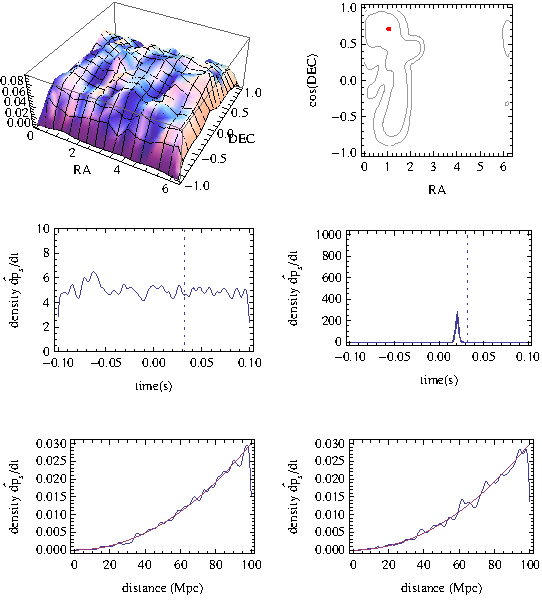
\includegraphics{Figures/fig-mma-DemoSampler.pdf}
\caption{\label{fig:Milestones:DemoSampler:Mathematica}\textbf{Example sampler results (Mathematica)}: Example of a
  uniform sampler (left) and time-of-flight-targeted sampler (right).  Plots show the sky position distribution (top);
  time distribution (center); and distance distribution (right). 
}
\end{figure*}

\noindent \textbf{Time-of-flight sampler}: Generate random arrival times; convert to a sky position and arrival time.
Examples of these samplers are shown in Figure \ref{fig:Milestones:DemoSampler:Mathematica}.
\begin{itemize}
\item \emph{Inversion tests}: Confirm the low-level time-of-flight code, given time of flights derived from a sky
  location and time, recover that sky location and time.
\item \emph{Sampling distribution}: Plot a sampling distribution in $\hat{n}$ and $t$ derived from a random location. 

 Confirm the location improves (and  converges to the point and mirror point) as the timing errors decrease.
\end{itemize}

\subsection{Milestones and Benchmarks:  Intrinsic exploration (*)}

\noindent \textbf{Document prototype exploration procedure}: Trigger values to seed mass range? Fisher matrix?


\noindent \textbf{Implement, demonstrate serial code}: Just do it





\end{widetext}
\subsection{Requirements}

\noindent \textbf{GraceDB event rate}: Processing time needed for realtime followup is roughly 1/hour.

\noindent \textbf{Operation count}: Fortunately the huge data set is only processed once to generate a \emph{very small}
set of intermediate quantities.  After a few O(N) operations, the \emph{actionable} memory usage is very small


\noindent \textbf{Memory usage: Computation}: A stupid approach is to use a fixed sampling rate for all time.
%
A 30 min signal at 4kHz with 3 detector REAL8 timeseries $\simeq 180 Mb$.
%% << PhysicalConstants`
%% 30 Minute * 4096/Second * 3 * 8 Byte
%% Convert[%, Mega Byte] // N
Plus, we \textbf{must} create each harmonic tineseries -- with 5 harmonics, this is Gb of storage!  (Plus a factor of few for intermediate
data: the FFTs.)

\noindent \emph{Compressing in time-frequency}: A better approach to the likelihood only evaluates the terms we need.
Memory usage should be \emph{much} more moderate if we only evaluate a handful of inner products. uses (a) tapered sampling rates in
the raw data and template or (b) some intelligent representation (e.g., amplitude-phase representations for the $h_{lm}(f)$).

\noindent \textbf{Memory usage: Output}: 

\noindent \textbf{File I/O} \editremark{don't know} how fast the current disk speeds are, NFS limits, interconnect, etc


\subsection{Routines needed}

\noindent \textbf{Distribution infrastructure}: To evaluate $\int L p$ and $\int p_s L p/p_s$, we first need to define
a distribution object and require certain features:

* request bound on each parameter (e.g., could identify 'light ring normal' and 'light ring width'; 'time
window.barycenter', etc. )

* return random sample from each parameter

* return PDF


\noindent \textbf{Monte carlo integrator}: In terms of $p_s$

* Monte carlo integrator with convergence test (i.e., threshold on $L_{\rm reduced}$ and error tolerance target,
absolute and relative)

** ideally ability to multithread


\noindent \textbf{Ldata and Lsignal}: 



\subsection{Code tests}




\section{Stage 2: Short-term deliverables and selling points (*)} 

\subsection{Results(*)}

\noindent \textbf{Intrinsic mass posterior:}

\noindent \textbf{Reliability of confidence contours}: To demonstrate confidence in each one-dimensional posterior, for
each simulated event $\alpha$ and coordinate $A$ we evaluate the one-dimensional cumulative distribution $P_{\alpha,A}$
and in particular this scalar evaluated at the injection location [$P_{\alpha,A}(x_{\alpha,A})$].  

As an example Figure \ref{fig:ShortTermDemo:OneDCumulativeInjectionRecovery} shows our confidence distribution.
The sources in the sample were drawn randomly from the same prior used \editremark{XXX}

\noindent \textbf{Evidence:}



\begin{figure}
\caption{\textbf{Example of two-dimensional posterior $p(m_1,m_2)$}:
}
\end{figure}

\begin{figure}
\caption{\label{fig:ShortTermDemo:OneDCumulativeInjectionRecovery}\textbf{Example of confidence in confidence
    intervals}: The cumulative distribution of $P_{\alpha,A}(x_{\alpha,A})$ for several variables $A$: chirp mass; mass
  ratio $\eta$; sky location RA; sky location DEC \editremark{do all?}
}
\end{figure}

\subsection{Selling points}

\begin{verbatim}
 -low-latency
 -evidence accurate
 -modular: infrastructure compatible with other uses
\end{verbatim}



\section{Stage N-2: Mid-term deliverables  (*)}
\subsection{Quantity is a quality all its own}
Our speed and performance allow lar

\subsubsection{Revisit prior studies}

\noindent \textbf{Fisher matrix breakdown?}: Ilya et al claim the Fisher matrix breaks down for some noise realizations
with moderate SNR.  That's plausible but it'd be nicce to better understand why.  And to be \emph{confident} it's not a
convergence issue.

\subsubsection{New studies}


\section{Stage N-1: Mid-term technical issues (*)}

\noindent \textbf{SNR and breakdowns}: At high SNR, we can \emph{easily} have timing resolution smaller than our
sampling rate (unless using 16 kHz). 

If the SNR is above the low tens, nongaussianities will occur as a matter of course .  [This might in part explain the
  non-Fisher-matrix claims made above.]

\noindent \textbf{PSD sensitivity}: How do we handle the smoothing (1/30 minute  frequency bins?)



\section{Stage N: Long term speculations (*)}


\subsection{Search integration}

\noindent \textbf{As a final coherent stage}: Running with just $(2,\pm 2)$ modes on the triggered masses (exact bank
coincidence) provides a final coherent stage with a confidence statistic (evidence).  Just saying.

If we use exact bank coincidence and a low-dimension $(l,m)$ space, the operations will be sub-minute (few seconds) --
allowing high trigger rates. \editremark{I wonder if this is useful}.



\part{Richard's notes to self}

\section{Python implementation}

\noindent \textbf{Input check}: 

* I use the raw $h_{lm}(t)$ in my mathematica code -- it's fine

* $\tilde{h}_{lm(f)}$

* Fourier convention: $\tilde{h}_{22}$ should have only positive frequencies \editremark{checkme}

\noindent \textbf{Operations check}

* make sure frequencies are consistently set EVERYWHERE.  It's very important to get all the PSD integrals using a
consistent lower frequency! \editremark{FIX ME}

\noindent \textbf{Intermediate structures}



* $Q$ timeseries has broad support

* \textbf{Distance scaling} incorrectx

\section{Mathematica implementation}

\noindent \textbf{Mathematica memory usage}: Huge overhead for arrays.  Calibrate usage for frame files and control
memory bloat

\noindent \textbf{Triangulation sampler}: Implement!

\noindent \textbf{Mass-dependent data length?}: Change data length depending on trigger chirp mass to reduce computation time.


\noindent \textbf{Converter}: Dump to quasi-MCMC output (\texttt{BayesianInport})

\section{Python implementaiton}

\noindent \textbf{Serial pipeline}: Rather than parallelize across the cluster, do a full zero-spin serial operation.
It will be easier to document the physics and infrastructure if it's in one code.

Make $L_{\rm marg}(m_1,m_2)$, recovery $p-p$ plots, etc

\noindent \textbf{Serial sky localization code}: Test our comparison against Bayesstar

\noindent \textbf{Mass-dependent data length?}: Change data length depending on trigger chirp mass to reduce computation time.



\appendix
\section{Gravy issues: Things to think about but not critical now}

% http://www.physics.gla.ac.uk/igr/GWbursts2012/pages/program/slides/MondayPM/Favata.pdf
\emph{Physics check 1: Memory modes}: The $m=0$ memory modes \cite{2009PhRvD..80b4002F,2009ApJ...696L.159F,2010CQGra..27h4036F,2011PhRvD..84l4013F} aren't consistently implemented: present with
  TaylorTN but \emph{not} with SpinTaylorT4.   If they \emph{are}
  implemented, their spectrum is \textbf{incredibly sensitive to numerical effects: start and particularly the abrupt
    end of the signal}.  Finally, memory is \textbf{physically incompatible with zero padding}: we need to ``pad and
  extend'', not zero pad!    But for non-IMR waveforms, we don't know how to do that without \textbf{explicitly} knowing
  which parts of the signal are memory!

Do you care?  Memory modes are \emph{not} always sufficiently insignificant: if the signal is short and the number of cycles
$N_{c}$ is small compared to $1/\rho^2$, then these overlaps matter:
\begin{eqnarray}
\qmstateproduct{h_{22}}{h_{20}} \simeq O(1) \times \qmstateproduct{h_{22}}{h_{22}}/N_c 
\end{eqnarray}
You should confirm these overlaps are \emph{not} zero with \texttt{TaylorT4} but \emph{are} zero for
\texttt{SpinTaylorT4} (when implemented).

\textbf{Should we fix it now?} No.  It's a relatively minor fix; everyone made this mistake; it's less important for
long aLIGO waveforms. \editremark{Gravy item for the paper}

\textbf{Should we manually set m=0 modes to zero for nonprecessing?}: Not yet...

\begin{shaded}
\noindent \textbf{Gravitational wave memory}: One informal   ad-hoc argument suggesting significant memory ($\tilde{h}(f)\propto f^{-1}$)
  relies on $h$ changing by a nonzero amount in the $(l,0)$ modes.    These discontinuities are inevitable consequences
  of radiation and insure $\tilde{h}$ decays as $1/f$ at high frequency.

\noindent \textbf{Do we implement it?}: Nope.  And what we do implement is seriously broken

\noindent \textbf{How can we fix it?}

\noindent \textbf{What are the physical consequences of memory modes?}: The memory modes have nonzero overlap with
everything. [For a nonprecessing binary, $\tilde{h}^{\rm mem} \simeq i \Delta h/2\pi f$ below a characteristic cutoff
scale (i.e., the merger timescale).]
\end{shaded}
\section{Notation issues: Comparing with standard notation}

\subsection{Signal amplitude}

\noindent \textbf{Single-interferometer: Complex notation}
For a single perpendicular-arm detector with waves \emph{propagating from} $\hat{n}=n(\theta,\phi)$ on the sky and with
polarization angle $\psi$ \emph{along that direction} \editremark{check signs}
\begin{subequations}
\label{eq:SingleIFOResponse}
\begin{eqnarray}
\begin{bmatrix}
F_+ \\ F_\times 
\end{bmatrix}
&=& \begin{bmatrix}
e_+(z):e_+^{(gw)}(-\hat{n},\psi) \\
e_+:e_\times^{(gw)} 
\end{bmatrix}
 \\
&=& 
\begin{bmatrix}
\cos 2\psi & \sin 2 \psi \\
- \sin 2 \psi & \cos 2 \psi
\end{bmatrix}
\begin{bmatrix}
\frac{1}{2} (1+\cos^2\theta) \cos2\phi  \\
\cos \theta \sin 2 \phi
\end{bmatrix} \nonumber
\\
F_\mathrm{+} &=&
 \frac{1}{2}(1+\cos^{2} \theta) \cos 2 \phi \cos 2 \psi
\nonumber\\ &+& \cos \theta \sin 2 \phi \sin 2 \psi \, \\ 
F_\mathrm{\times} &=&- \frac{1}{2}(1+\cos^{2} \theta) \sin 2 \phi \cos 2 \psi
\nonumber \\ &+& \cos \theta \cos 2 \phi \sin 2 \psi
\end{eqnarray}
\end{subequations}
where $e_+^{(gw)}$ are the appropriately rotation-modified structures
previously and $\psi$ is a polarization orientation (i.e., the third
euler angle associated with the rotation operator; see the SU(2) reference).  
%
In the text it will be helpful to express them in complex form:
\begin{eqnarray}
{} [F_{+}+i F_{\times}](\hat{n},\psi) &=& \frac{\sqrt{4\pi}}{\sqrt{5}}\left[ e^{-2i\psi}\Y{-2}_{22} +
  e^{+2i\psi}\Y{-2}_{2,-2}  \right] 
\end{eqnarray}


\noindent \textbf{Conventional signal amplitude expression}: 
A nonprecessing source dominated by a single pair of conjugate $(2,\pm 2)$ modes has a simple signal and a well-known
signal-to-noise ratio expression.  That standard expression (replacing $\iota \rightarrow \theta_E$ and $\phi_c \rightarrow \phi_E$) has the
following form \editremark{signs certainly wrong}
\begin{subequations}
\label{eq:SingleIFO:AmplitudeSquared}
\begin{align}
H_1 &= F_+(\theta_S,\phi_s,0) h_+ + F_\times(\theta_S,\phi_S,0)h_\times \\
    &= \text{Re} (F_++i F_\times) e^{-2i\psi} [\frac{1+\cos \theta^2_E}{2}h_{+,\hat{z}} - i \cos \theta_S
  h_{\times,\hat{z}}] \\
 &= {\cal F}_+ h_{+,\hat{z}} + {\cal F}_{\times} h_{\times, \hat{z}} \\
{\cal F}_+ &= F_+(\theta_S,\phi_S,\psi)\frac{ 1+\cos^2 \theta_E}{2} + F_\times(\theta_S,\phi_S,\psi) \cos \theta_E \\
{\cal F}_\times &= F_\times(\theta_S,\phi_S,\psi) \cos \theta_E  + F_+(\theta_S,\phi_S,\psi)\frac{1+\cos^2\theta}{2}\\
\end{align}
where we absorb inclination and polarization dependence into the generalized detector response functions ${\cal F}$.
Substituting into the signal amplitude expression and using orthogonality and equal amplitude of $h_{+,\hat{z}}$ and $h_{\times, \hat{z}}$:
\begin{align}
\qmstateproduct{H_1}{H_1}_1 
  &= \qmstateproduct{h_{+,z}}{h_+,z} [{\cal F}_+^2  + {\cal F}_\times^2]
% \text{Re}[(F_++i F_\times) e^{-2i\psi} \frac{1+\cos^2 \theta_E}{2}]^2 \nonumber \\ & 
%+  \text{Im}[(F_++i F_\times) e^{-2i\psi} \cos \theta_E]^2
\end{align}
\end{subequations}

\section{Extensions and comparison: F statistic}

In GW searches,  polarization phase marginalization can be done simultaneously.  At each timesample, we expected we could
 marginalize \emph{analytically} over polarization phase, with a bessel function. 


\subsection{Marginalizing in the polarization angle}

\begin{shaded}
\noindent \textbf{Template amplitude}: Using the $\sigma,\epsilon$ notation of \citet{CutlerFlanagan:1994}, the signal amplitude term has the form $\rho^2 = \sigma
\rho_0^2(1+\epsilon \cos 4(\psi-\psi_0))$ where $\rho_0^2$ is the amplitude of a source directly overhead a single
detector and $\sigma,\epsilon$ are derived from the beampattern functions:
\begin{eqnarray}
C_{\lambda \lambda'}&=& \sum_k \begin{bmatrix}
F_+^2 & F_+F_\times \\
F_\times F_+ & F_\times^2
\end{bmatrix}\\
&=& \sum_k [P_k : \hat{e}_\lambda(\hat{n})] [P_k : \hat{e}_{\lambda'}(\hat{n})]  \nonumber \\
& =& \sigma U\begin{bmatrix} (1+\epsilon) & 0 \\ 0 & 1-\epsilon \end{bmatrix} U^{-1} 
\end{eqnarray}
where $U$ is a unitary transformation that diagonalizes $C$.

\noindent \textbf{Response against data}: By contrast, for a fixed data set, the second term in the likelihood
necessarily transforms like $h$: purely sinusoidally in polarization angle
\begin{eqnarray}
\rho \hat{\rho} = A \cos 2\psi + B \cos 2 \psi
\end{eqnarray}
\noindent \textbf{Marginalizing?}: If this were the only term in the likelihood -- for example, for an isotropic network
--  we could marginalize exactly: \textbf{BUT THIS IS NOT TRUE}
\begin{align}
\ln L  &= [\ln L]_c \cos 2\psi + [\ln L]_s \sin 2\psi = \ln L_0 \cos 2(\psi-\psi_0)  \\
\ln L_0 &= \sqrt{[\ln L]_c^2+[\ln L]_c^2} \\
\int_0^{\pi}\frac{ d\psi}{\pi} L &= \frac{1}{\pi}I_0(\ln L_0)
\end{align}
In general $\rho$ depends on $\psi$, so we can't: both $\cos 2\phi$ and $\cos 4\psi$ appear in the exponential, unless
the network has $\epsilon=0$ (i.e., equal sensitivity to both polarizations).
\end{shaded}



\subsection{F statistic}

When viewed as maximization, this approach resembles the F statistic
\cite{1998PhRvD..58f3001J,2005PhRvD..72f3006C,2012PhRvD..86l3010K,gwastro-HarryFairhurst-CoherentTargetedSearch}\cite{BCV:PTF}.



\noindent \textbf{F statistic versus our approach}: The F statistic approach uses 4 real basis functions (2 polarizations
plus cosine, sine chirp in each).  Including distance, these 4 basis functions have arbitrary coefficients in each
signal: all possible realizations exist and correspond to different physical configurations with different
$(d,\theta_S,\phi_S,\psi)$.  Maximization (or marginalization) of the likelihood over these four amplitudes is possible
analytically! Why? Because the likelihood  $-\rho^2/2 + \ln L_{\rm data}$ has the form \editremark{roughly speaking}
\begin{eqnarray}
\ln L \propto a_\alpha \sum_k\qmstateproduct{h_\alpha}{\hat{H}_k}_k + a_\alpha a_\beta \qmstateproduct{h_{\alpha}}{h_\beta}_k
\end{eqnarray}
which, modulo measure factors, can be marginalized via gaussian integral tricks.

In our approach,  more than 4 real basis functions exist.  Their amplitudes are \textbf{not independent}, because there
are more than 4 of them (but still only 4 real-valued parameters). 

Additionally, in our approach, \textbf{the sine and cosine chirp are not exactly orthgonal, and we have memory modes}
(in general).  This effect is noticable in iLIGO-scale (short) signals

 The F-statistic trick is a possible \emph{approximation} but not valid in general, particularly  not  for precessing binaries




\bibliography{overviewexport}
\end{document}

